\documentclass{article}
%-------------------------------------------------------
\usepackage{graphicx}
\usepackage{subcaption}
\usepackage{amsmath}
%-------------------------------------------------------
\begin{document}
%-------------------------------------------------------
\title{Flyback Converter Design and Analysis}
\author{Mohamed Gueni}
\date{\today}
%-------------------------------------------------------
\maketitle
%-------------------------------------------------------
\tableofcontents
%-------------------------------------------------------

\section{Introduction}
A flyback converter is a type of DC-DC converter widely used in applications requiring a single output voltage and galvanic isolation between input and output. This document details the design of a single-output flyback converter with a 25V DC input and a 12V DC output. The converter includes an RC snubber and an RCD clamp to handle switching transients and protect the components.

\section{System Diagram}
%-------------------------------------------------------
\begin{figure}[htbp]
    \centering
    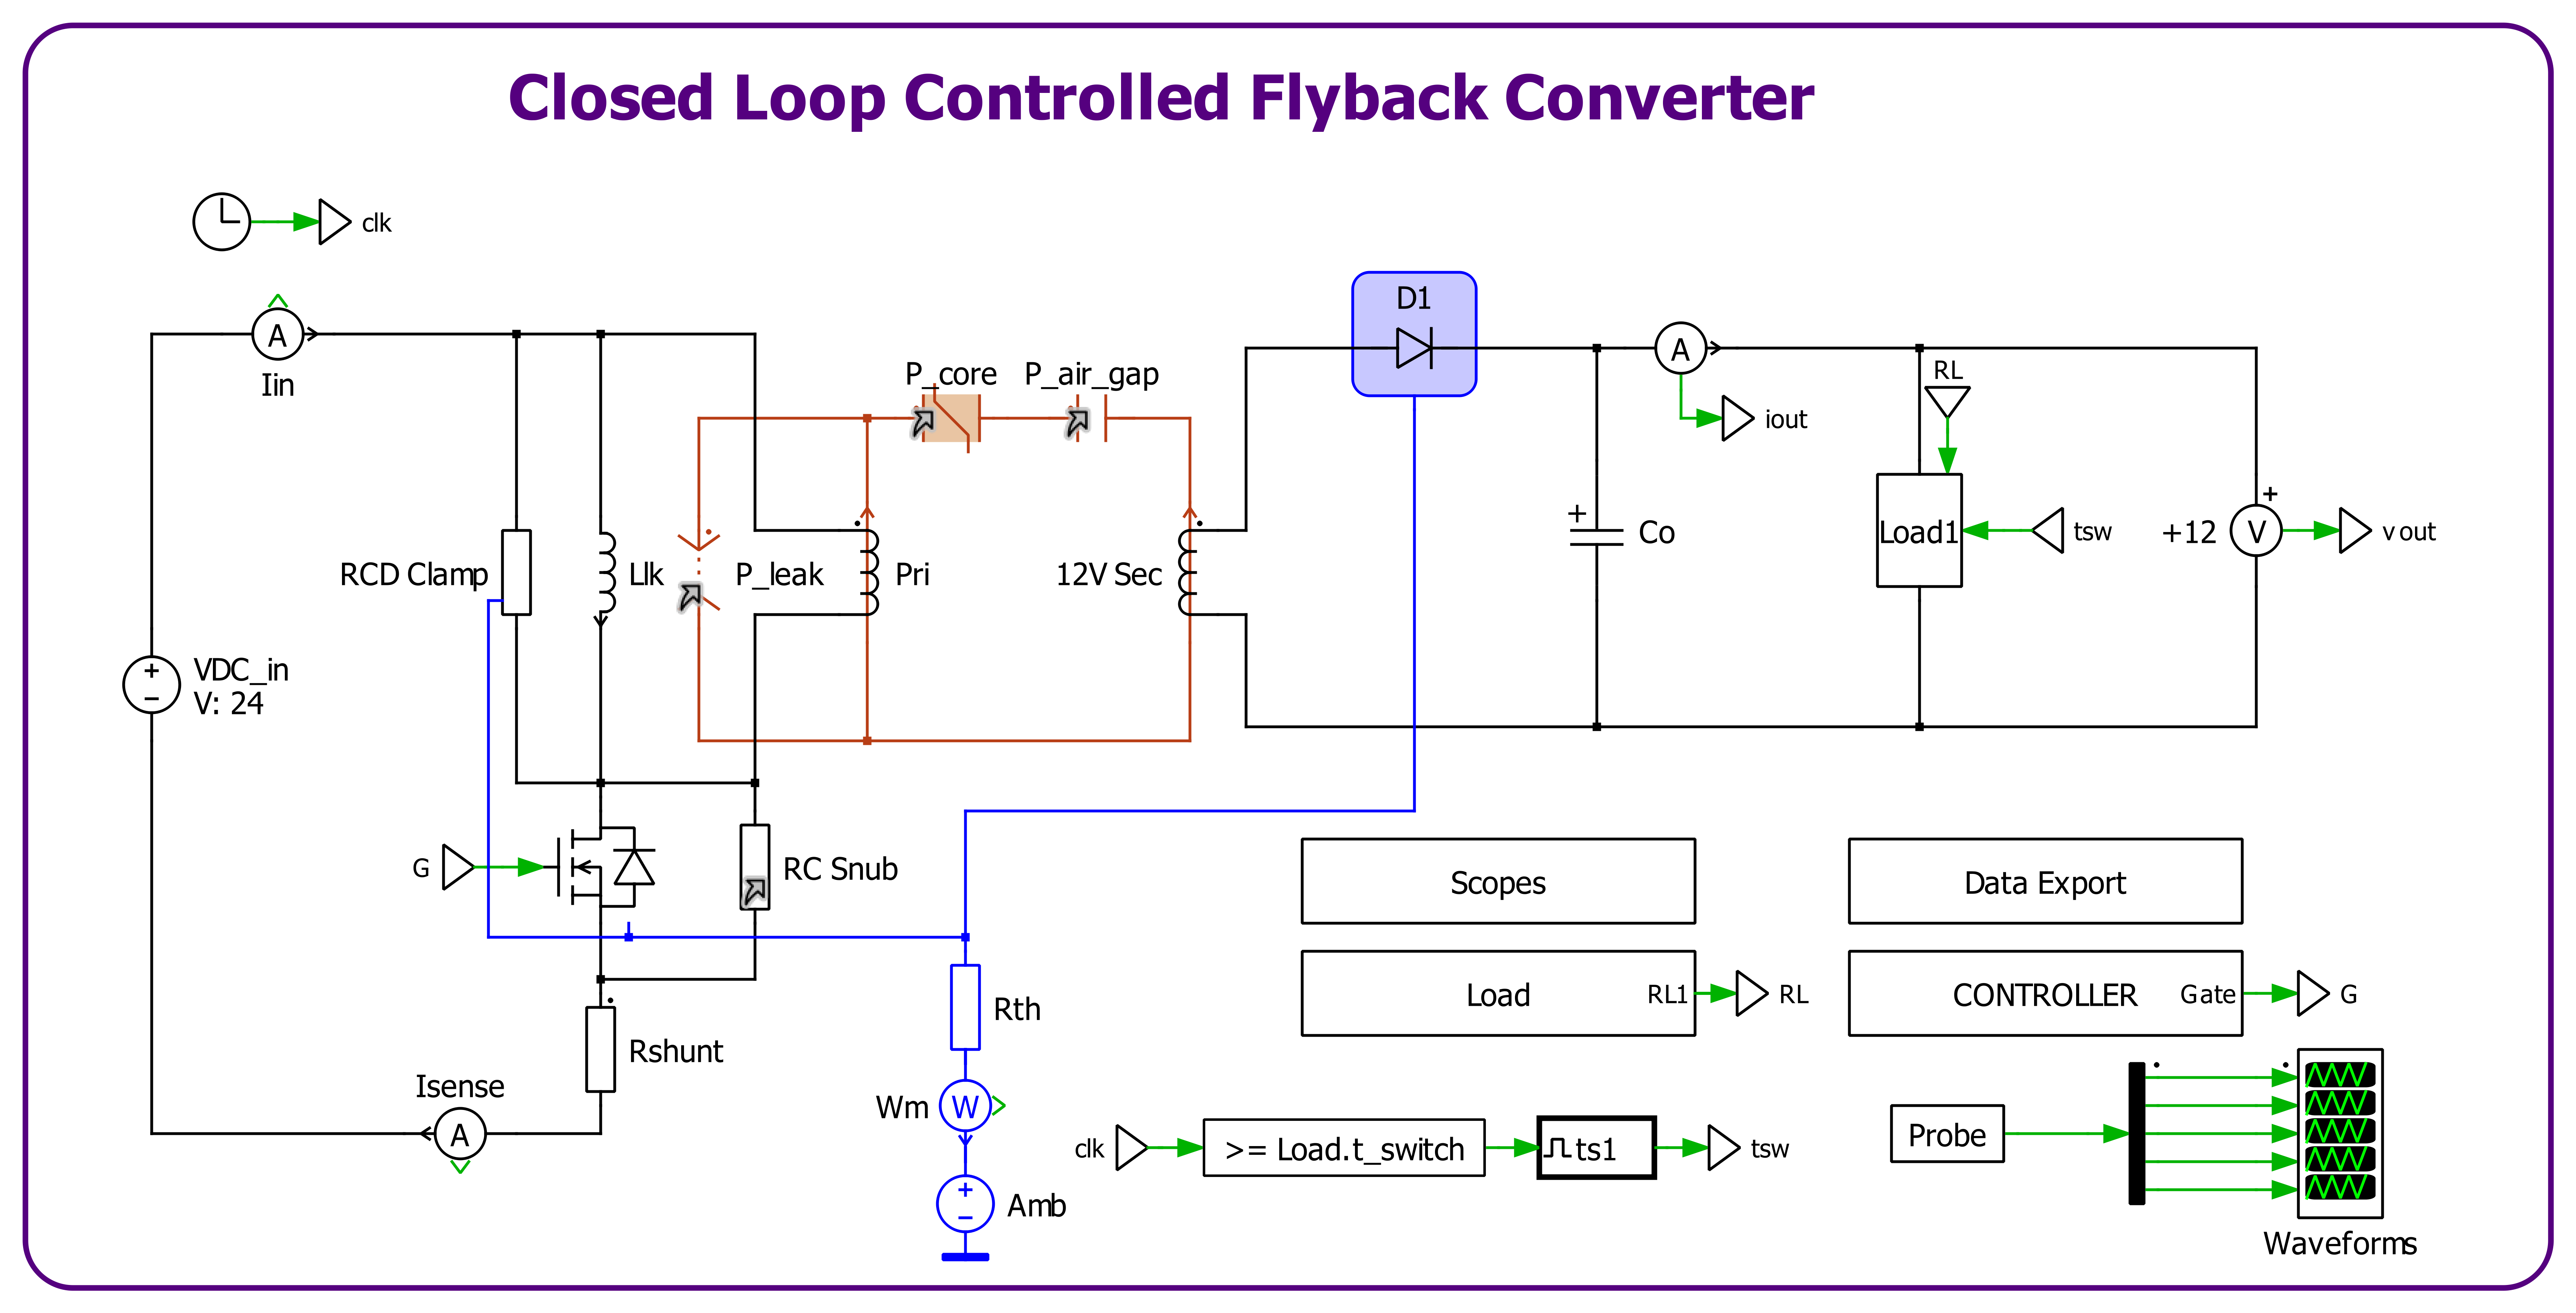
\includegraphics[width=\textwidth]{flyback.jpg}
    \caption{Flyback Converter System Diagram}
    \label{fig:Flyback}
\end{figure}
%-------------------------------------------------------

\section{System Description}
The flyback converter operates by storing energy in a transformer during the switch-on period and releasing it to the output during the switch-off period. This section elaborates on each part of the system.

\subsection{Transformer}
The transformer in a flyback converter serves two primary purposes:
\begin{itemize}
    \item **Energy Storage and Transfer**: During the switch-on period, energy is stored in the transformer's magnetic field. During the switch-off period, this energy is transferred to the output.
    \item **Voltage Transformation and Isolation**: The transformer steps down the input voltage to the required output level and provides galvanic isolation between the input and the output.
\end{itemize}

\subsubsection{Turns Ratio Calculation}
The turns ratio is calculated to meet the output voltage requirements based on the input voltage and the desired duty cycle.

\[
\frac{N_{pri}}{N_{sec}} = \frac{V_{out} + V_{f}}{V_{in} \times D_{max}}
\]

Where:
\begin{itemize}
    \item $N_{pri}$ is the number of turns on the primary winding.
    \item $N_{sec}$ is the number of turns on the secondary winding.
    \item $V_{f}$ is the forward voltage drop of the diode.
    \item $D_{max}$ is the maximum duty cycle, typically 0.4 to 0.6 for flyback converters.
\end{itemize}

\subsubsection{Primary Inductance}
The primary inductance $L_{pri}$ is crucial for determining the converter’s mode of operation. For continuous conduction mode (CCM), $L_{pri}$ must be sufficiently large.

\[
L_{pri} = \frac{V_{in} \times D_{max} \times (1 - D_{max})}{f_s \times I_{pri, peak}}
\]

Where:
\begin{itemize}
    \item $I_{pri, peak}$ is the peak current through the primary winding.
    \item $f_s$ is the switching frequency.
\end{itemize}

\subsubsection{Core Selection}
The core material and size are selected based on the required inductance and the peak magnetic flux density ($B_{max}$).

\[
B_{max} = \frac{V_{in} \times D_{max}}{N_{pri} \times A_e \times f_s}
\]

Where:
\begin{itemize}
    \item $A_e$ is the effective core area.
\end{itemize}

\subsection{Output Rectification and Filtering}
The output rectification and filtering stages convert the AC voltage from the transformer's secondary winding into DC voltage and reduce voltage ripple.

\subsubsection{Output Diode}
The diode rectifies the AC voltage from the transformer into DC. It must be selected based on its peak reverse voltage and average forward current ratings.

\[
V_{R, peak} = V_{in} + V_{out} \times \frac{N_{pri}}{N_{sec}}
\]

\[
I_{avg} = \frac{P_{out}}{V_{out}}
\]

Where:
\begin{itemize}
    \item $V_{R, peak}$ is the peak reverse voltage the diode must withstand.
    \item $I_{avg}$ is the average current the diode must carry.
\end{itemize}

\subsubsection{Output Capacitor}
The capacitor filters the rectified voltage to reduce ripple and provide a stable DC output.

\[
C_{out} = \frac{I_{out} \times D_{max}}{f_s \times \Delta V_{out}}
\]

Where:
\begin{itemize}
    \item $I_{out}$ is the output current.
    \item $\Delta V_{out}$ is the allowable ripple voltage.
\end{itemize}

\subsection{RC Snubber Circuit}
The RC snubber circuit is used to dampen oscillations caused by the transformer's leakage inductance during the switching transitions.

\subsubsection{Purpose of the RC Snubber}
The RC snubber protects the MOSFET switch from voltage spikes and reduces EMI by damping high-frequency oscillations.

\subsubsection{Snubber Resistor and Capacitor Calculation}
The resistor and capacitor in the snubber circuit are chosen to critically dampen the oscillations.

\[
R_s = \sqrt{\frac{L_{leak}}{C_s}}
\]

\[
C_s = \frac{1}{2 \pi \times f_{ring} \times R_s}
\]

Where:
\begin{itemize}
    \item $L_{leak}$ is the leakage inductance of the transformer.
    \item $f_{ring}$ is the ringing frequency, typically a few MHz.
\end{itemize}

\subsection{RCD Clamp Circuit}
The RCD (Resistor-Capacitor-Diode) clamp circuit limits the peak voltage across the MOSFET by diverting excess energy from the leakage inductance.

\subsubsection{Purpose of the RCD Clamp}
The RCD clamp prevents the MOSFET from being damaged by voltage spikes due to the transformer's leakage inductance.

\subsubsection{Clamp Resistor and Capacitor Calculation}
The clamp resistor dissipates the energy stored in the leakage inductance, and the capacitor stores the energy to limit voltage spikes.

\[
R_{clamp} = \frac{V_{clamp} - V_{in}}{I_{leak}}
\]

\[
C_{clamp} = \frac{\Delta E}{\Delta V_{clamp}^2}
\]

Where:
\begin{itemize}
    \item $V_{clamp}$ is the clamping voltage.
    \item $\Delta E$ is the energy stored in the leakage inductance.
    \item $\Delta V_{clamp}$ is the allowable voltage ripple on the clamp capacitor.
\end{itemize}


\section*{Reverse Polarity Protection}
%-------------------------------------------------------
\begin{figure}[htbp]
    \centering
    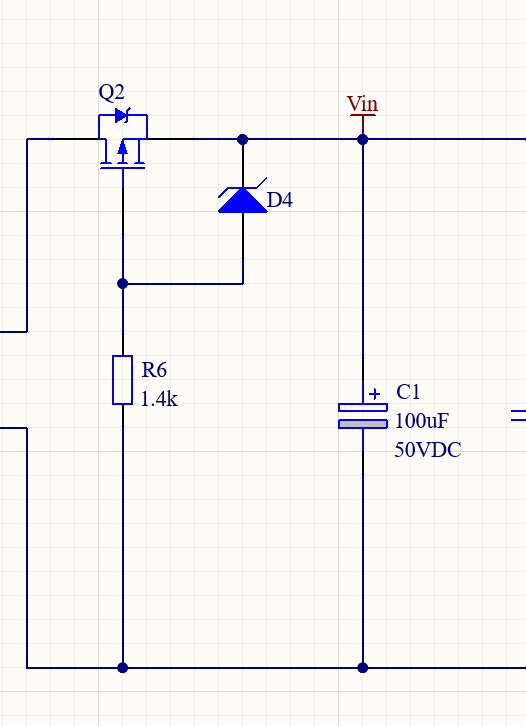
\includegraphics[width=\textwidth]{RVP.png}
    \caption{Reverse Polarity Protection}
    \label{fig:RVP}
\end{figure}
%-------------------------------------------------------
When the input is connected correctly (positive to the source of the PMOS and negative to the drain), the PMOS will be in the ON state, allowing current to flow. If the polarity is reversed, the PMOS remains OFF, preventing current from flowing and protecting your circuit. 

Below is a step-by-step guide on how to choose these components:

\subsection*{1. Selecting the PMOS Transistor}

\begin{itemize}
    \item \textbf{Voltage Rating (V\(_{DS}\)):} The PMOS should have a drain-source voltage rating higher than the maximum input voltage. Since the input can go up to 36V, a PMOS with at least 40V V\(_{DS}\) rating is good to provide a margin.
    
    \item \textbf{Current Rating (I\(_{D}\)):} The PMOS must handle the maximum current drawn by your circuit. Since the circuit could draw more than 2A, we choose a PMOS with a current rating higher than 2A, preferably 5A or more for safety.
    
    \item \textbf{R\(_{DS(on)}\):} This is the on-state resistance of the PMOS when it's fully turned on. Lower R\(_{DS(on)}\) values reduce power loss and heat dissipation. Usually a PMOS with R\(_{DS(on)}\) in the range of a few milliohms (m\(\Omega\)).
\end{itemize}

\subsection*{2. Selecting the Zener Diode}

\begin{itemize}
    \item \textbf{Zener Voltage (V\(_Z\)):} The Zener diode is used to ensure the gate-source voltage (V\(_{GS}\)) of the PMOS stays within safe limits. We go for a Zener voltage slightly higher than the PMOS gate threshold voltage (V\(_{GS(th)}\)) but lower than the maximum allowed V\(_{GS}\) for the PMOS.
    
    \item \textbf{For example:} If the PMOS has a V\(_{GS(th)}\) of -2V and a maximum V\(_{GS}\) of -20V, we could choose a Zener diode with a V\(_Z\) of 10V. This ensures the gate is clamped to a voltage that fully turns on the PMOS but doesn’t exceed the maximum V\(_{GS}\).
\end{itemize}

\subsection*{3. Selecting the Resistor}

\begin{itemize}
    \item \textbf{Resistor Value (R):} The resistor is used to limit the current flowing through the Zener diode and to ensure that the PMOS gate is pulled to the source ground when the input is connected with the correct polarity.
    
    \item \textbf{Calculation:} The resistor value can be calculated using Ohm's Law:
    \[
    R = \frac{V_{in} - V_{Z}}{I_{Z}}
    \]
    Where \(V_{in}\) is the input voltage, \(V_{Z}\) is the Zener voltage, and \(I_{Z}\) is the Zener current, which should be enough to activate the Zener diode but not too high to damage it (typically in the range of 5-20mA).
    
    \item \textbf{Example:} in this case we chose a Zener with a 10V rating and want a current of 10mA, and the input voltage is 24V, the resistor then value would be:
    \[
    R = \frac{24V - 10V}{10mA} = 1.4k\Omega
    \]
\end{itemize}

\section{References}

\begin{enumerate}
    \item R. W. Erickson, \textit{Fundamentals of Power Electronics}, New York: Chapman \& Hall, 1997.
\end{enumerate}

\section{Units}

\begin{enumerate}
    \item Farads (\textbf{F}).................: Unit of capacitance.
    \item Amps (\textbf{A})..................: Unit of electric current.
    \item Volts (\textbf{V})...................: Unit of electric potential.
    \item Ohms (\textbf{$\Omega$})............: Unit of electrical resistance.
    \item Henrys (\textbf{H}).................: Unit of inductance.
    \item Watts (\textbf{W}).................: Unit of power.
    \item Hertz (\textbf{Hz}).................: Unit of frequency.
    \item Teslas (\textbf{T})...................: Unit of magnetic flux density.
    \item Webers (\textbf{Wb}).............: Unit of magnetic flux.
    \item Decibels (\textbf{dB}).............: Unit of measurement for the power level of an electrical signal.
\end{enumerate}

%-------------------------------------------------------
\end{document}
%-------------------------------------------------------
